\documentclass[a4paper,12pt]{book}

%Template per documenti e tesi

\usepackage[utf8]{inputenc}
\usepackage[italian]{babel}
\usepackage{float}
\usepackage{graphicx}
\usepackage[left=2.5cm,right=2.5cm,top=3cm,bottom=3cm]{geometry}
\usepackage{hyperref}
\usepackage{setspace}
\usepackage{shapepar}
\usepackage{listings}
\usepackage[table,xcdraw]{xcolor}
\usepackage{fonttable}
\usepackage{amssymb}
\usepackage{amsmath}
%\usepackage{enumerate}
%\usepackage{enumitem}
\usepackage{fontawesome}

\usepackage{color} %red, green, blue, yellow, cyan, magenta, black, white
\definecolor{mygreen}{RGB}{28,172,0} % color values Red, Green, Blue
\definecolor{mylilas}{RGB}{170,55,241}

\colorlet{punct}{red!60!black}
\definecolor{background}{HTML}{EEEEEE}
\definecolor{delim}{RGB}{20,105,176}
\colorlet{numb}{magenta!60!black}
\definecolor{dkgreen}{rgb}{0,0.6,0}
\definecolor{gray}{rgb}{0.5,0.5,0.5}
\definecolor{mauve}{rgb}{0.58,0,0.82}

\lstset{frame=tb,
	language=Java,
	%aboveskip=3mm,
	%belowskip=3mm,
	showstringspaces=false,
	columns=flexible,
	basicstyle=\small\ttfamily,
	numbers=none,
	numberstyle=\scriptsize,
	keywordstyle=\color{blue},
	commentstyle=\color{dkgreen},
	stringstyle=\color{mauve},
	breaklines=true,
	breakatwhitespace=true,
	tabsize=3
}

\lstdefinelanguage{json}{
	basicstyle=\small\ttfamily,
	numbers=left,
	numberstyle=\scriptsize,
	stepnumber=1,
	numbersep=8pt,
	showstringspaces=false,
	breaklines=true,
	frame=lines,
	backgroundcolor=\color{background},
}

\hypersetup{
	colorlinks=false,
	linktoc=all, %both sections and subsections linked
}

\usepackage[hyperref,backend=bibtex,backref,backrefstyle=none,sorting=none]{biblatex}
\addbibresource{references.bib}
\usepackage{fancyhdr}

\newcommand{\makelogo}{%
	\centering
	\textsc{Università degli Studi di Napoli Federico II}
	\\[.4cm]
	\textsc{Dipartimento di Ingegneria Elettrica e Tecnologie dell'Informazione}
	\\[1.1cm]
	\includegraphics[width=0.7\textwidth]{./figures/logo_blu.png}\\[1.1cm]
	\textsc{Corso di Laurea Magistrale in Informatica\\A.A. 2017-18}
	\\[2.5cm]
	\textbf{Progetto Basi di Dati II Modulo B}
	\vfill
	%\end{par}
	\centering
	\begin{par}
		\begin{tabular}{lllll}
			& \textbf{Autori} &                        &  &  \\
			\textbf{Bizzarri Flavio} & \textbf{}       & \textbf{Cuomo Daniele} &  &  \\
			\textbf{N97000281}       & \textbf{}       & \textbf{N97000270}     &  &  \\
			&                 &                        &  & 
		\end{tabular}
	
	\end{par}
	%\par
}

\fancyhead{}
\fancyhead[LO,LE]{\slshape\nouppercase\leftmark}
\cfoot{\thepage}

\pagestyle{fancy}

\DefineBibliographyStrings{italian}{%
	bibliography = {Riferimenti},
}

\begin{document}

	
	\onehalfspacing
	%\doublespacing use in case of emergency
	\author{F. Bizzarri, D. Cuomo}
	\title{Progetto Finale Basi di Dati II}
	
	{\frontmatter
		\let\cleardoublepage\clearpage{\makelogo}
		\thispagestyle{empty}
		
		\chapter*{\centering {\normalsize Sommario}}
TODOTODOTODOTODOTODOTODOTODOTODOTODOTODOTODOTODOTODOTODOTODOTODOTODOTODOTODOTODOTODOTODOTODOTODOTODOTODOTODOTODOTODOTODOTODOTODOTODOTODOTODOTODOTODOTODOTODOTODOTODO
Si vuole realizzare un data warehouse destinato all’analisi di dati riguardanti misurazioni effettuate su veicoli da parte dell’Istituto Motori di Napoli.
I dati in questione presentano anche la componente spaziale rappresentata dalle coordinate GPS dei rilevamenti.
Il DW realizzato è di tipo ROLAP, implementato con PostgreSQL, il quale fornisce sia tutte caratteristiche necessarie al data warehousing sia un’estensione spaziale.
		
		\tableofcontents
		
		\thispagestyle{empty}
		\mainmatter
	}
	
	
	\let\cleardoublepage\clearpage{		
		%\include{./chapters/intro}
		\chapter{Progettazione}

\section{Interrogazioni}
\begin{table}[h]
\begin{tabular}{cll}
	\rowcolor[HTML]{333333} 
	{\color[HTML]{FFFFFF} \#} & {\color[HTML]{FFFFFF} Query}                                                                                       & {\color[HTML]{FFFFFF} Obiettivo}                                                                                                                                                                                                                   \\
	1                         & \begin{tabular}[c]{@{}l@{}}Impatto ambientale medio in corse\\ da 5 km (CO2 e NOx, massa)\end{tabular}             & \begin{tabular}[c]{@{}l@{}}Pensata per analizzare varianti della\\ stessa interrogazione su diversi livelli\\ di granularità\end{tabular}                                                                                                          \\
	\rowcolor[HTML]{C0C0C0} 
	2                         & \begin{tabular}[c]{@{}l@{}}Consumo medio per intervalli di\\ velocità prefissati, su tutto il dataset\end{tabular} & \begin{tabular}[c]{@{}l@{}}Utile all'implementazione e l'analisi\\ di viste materializzate che\\ raggruppano i dati secondo delle \\ fasce di velocità. Le fasce scelte, \\ espresse in km/h, sono le seguenti:\\ 0-50, 50-90, 90-130\end{tabular} \\
	3                         & \begin{tabular}[c]{@{}l@{}}Efficienza dell'auto per intervalli\\ di RPM (rotazioni per minuto)\end{tabular}        & \begin{tabular}[c]{@{}l@{}}Altra interessante interrogazione\\ creata allo scopo di sfruttare le\\ viste materializzate. Il dataset \\ fornisce tutti i parametri \\ necessari al calcolo dell'efficienza, \\ o rendimento istantaneo\end{tabular} \\
	\rowcolor[HTML]{C0C0C0} 
	4                         & \begin{tabular}[c]{@{}l@{}}Per ogni test, media di NOx,\\ CO2, Potenza e Velocità\end{tabular}                     & \begin{tabular}[c]{@{}l@{}}Quest'interrogazione serve a\\ valutare le prestazioni ottenute\\ dall'esecuzione su di un \\ partizionamento verticale con le\\ colonne sparse tra più tabelle\end{tabular}                                            \\
	5                         & \begin{tabular}[c]{@{}l@{}}Media e deviazione standard\\ delle temperature\end{tabular}                            & \begin{tabular}[c]{@{}l@{}}Quest'interrogazione serve a \\ valutare le prestazioni ottenute\\ dall'esecuzione con le colonne \\ concentrate su di un unica\\ tabella restituita da un\\ partizionamento verticale\end{tabular}                    
\end{tabular}
\end{table}

\section{Diagrammi}
\begin{figure}
	\centering
	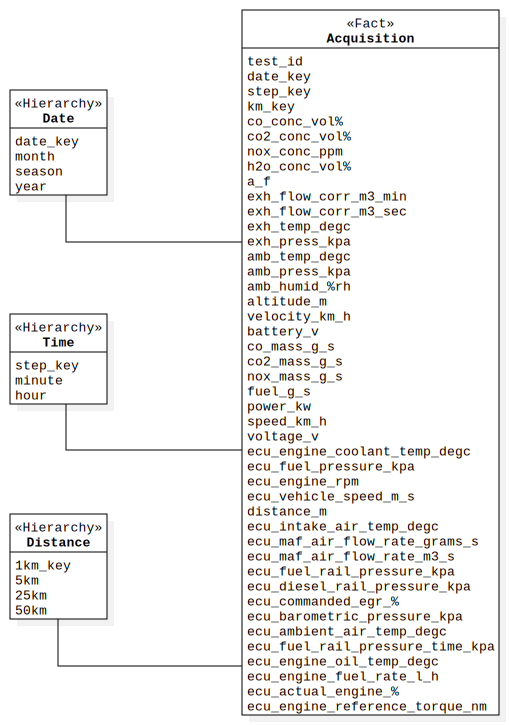
\includegraphics[width=1.\linewidth]{figures/class_fact_scheme}
	\caption{}
	\label{fig:ofm}
\end{figure}

		\chapter{Analisi}
In questo capitolo sono riportati i risultati e i tempi ottenuti per ogni fase: dalle procedure ETL all'esecuzione delle query.

\section{ETL}
\subsection{Trasformazione in CSV}
In questa sezione copriremo un'analisi dei tempi ottenuti nella fase che permette, a partire dai dati originali, di ottenere un file in formato CSV contenente i dati ripuliti da inconsistenze e in un formato adatto ad essere importato nel Datawarehouse.
In particolare nella fase di puliza, a partire dal file XSLX, si estraggono unicamente i record dove non appaiono valori negativi per quantità intrinsecamente positive (concentrazione, volume, ecc.); per i record ove manca il valore "relative" e/o la distanza percorsa si procede ad un calcolo a partire dall'ultima rilevazione valida estratta. Inoltre tutte le righe che presentano una chiara assenza di dati (70\% delle colonne) vengono scartate. Infine, durante la fase di trasformazione, per ogni file viene generata una data e un test\_id e per separare la parte intera da quella decimale si sostituisce la virgola con il punto.\\
I dati ottenuti si riferiscono ad una media aritmetica ottenuta testando 200 file ($\sim$1 milione di righe) generati a partire dal file originario fornito dall'Istituto Motori di Napoli.

\begin{table}[H]
	\centering
\begin{tabular}{ccccc}
	\rowcolor[HTML]{333333} 
	{\color[HTML]{FFFFFF}Righe XSLX}  
	& 
	{\color[HTML]{FFFFFF}Righe CSV}
	&
	{\color[HTML]{FFFFFF}Righe perse}
	&
	{\color[HTML]{FFFFFF}Peso file XSLX}
	&                                 
	{\color[HTML]{FFFFFF}Peso file CSV}\\
	\begin{tabular}[c]{@{}l@{}}5764\end{tabular}             
	& \begin{tabular}[c]{@{}l@{}}5706\end{tabular} 
	& \begin{tabular}[c]{@{}l@{}}1\%\end{tabular}  
	& \begin{tabular}[c]{@{}l@{}}2.138KB\end{tabular}  
	& \begin{tabular}[c]{@{}l@{}}2.283KB\end{tabular}   
\end{tabular}
\end{table}

\begin{table}[H]
	\centering
	\begin{tabular}{ccc}
		\rowcolor[HTML]{333333} 
	{\color[HTML]{FFFFFF}Fase di pulizia}
	&
	{\color[HTML]{FFFFFF}Fase di trasformazione}
	&
	{\color[HTML]{FFFFFF}Tempo totale}\\
	\begin{tabular}[c]{@{}l@{}}3.04s\end{tabular}             
	& \begin{tabular}[c]{@{}l@{}}0,05s\end{tabular} 
	& \begin{tabular}[c]{@{}l@{}}3,05s\end{tabular}
\end{tabular}
\end{table}

Questa fase mette in luce la buona qualità dei dati forniti dall'istituto: ci si aspetta in media di perdere pochissimi dati a causa di inconsistenze. Per quanto riguarda invece le dimensioni si nota come il formato Comma-separated values sia leggermente meno efficiente nella compressione rispetto al formato proprietario di Microsoft$^{\tiny{\textregistered}}$ ma al tempo stesso permetta una più veloce elaborazione.

\subsection{Import in tabella temporanea}
Al fine di importare i file CSV nella tabella dei fatti ci si appoggia ad una tabella temporanea al fine di agevolare le operazioni successive. Questa tabella viene troncata alla fine della procedura. L'import sfrutta la funzione \textit{COPY} messa a disposizione dal DBMS PostgreSQL.

\begin{table}[H]
	\centering
	\begin{tabular}{ccc}
		\rowcolor[HTML]{333333} 
		{\color[HTML]{FFFFFF}Numero file}
		&
		{\color[HTML]{FFFFFF}Numero righe}
		&
		{\color[HTML]{FFFFFF}Tempo}\\
		\begin{tabular}[c]{@{}l@{}}1\end{tabular}             
		& \begin{tabular}[c]{@{}l@{}}5706\end{tabular} 
		& \begin{tabular}[c]{@{}l@{}}214ms\end{tabular}\\
		\rowcolor[HTML]{C0C0C0}
		\begin{tabular}[c]{@{}l@{}}50\end{tabular}             
		& \begin{tabular}[c]{@{}l@{}}285.300\end{tabular} 
		& \begin{tabular}[c]{@{}l@{}}8,428s\end{tabular}\\
		\begin{tabular}[c]{@{}l@{}}100\end{tabular}             
		& \begin{tabular}[c]{@{}l@{}}570.600\end{tabular} 
		& \begin{tabular}[c]{@{}l@{}}16.522s\end{tabular}
	\end{tabular}
\caption{I dati si riferiscono ad una media di 5 esecuzioni}
\end{table}	
I risultati mostrano la bontà della funzione \textit{COPY} che sfruttando un inserimento batch di 1000 righe per volta riesce ad abbattere in modo consistente i tempi.

\subsection{Import nello schema}
In questa fase i dati, precedentemente inseriti in una tabella temporanea, vengono travasati nello schema proposto dopo aver disabilitato tutti gli indici. Le prove effettuate prendono in considerazione diverse dimensioni della tabella dei fatti oltre al caso in cui lo schema risulti partizionato.
\begin{table}[H]
	\centering
	\begin{tabular}{cccc}
		\rowcolor[HTML]{333333} 
		{\color[HTML]{FFFFFF}Dimensione tab. fatti}
		&
		{\color[HTML]{FFFFFF}Numero righe importate}
		&
		{\color[HTML]{FFFFFF}Partizionamento}
		&
		{\color[HTML]{FFFFFF}Tempo}\\
		\begin{tabular}[c]{@{}l@{}}0\end{tabular}             
		& \begin{tabular}[c]{@{}l@{}}285.300\end{tabular} 
		& \begin{tabular}[c]{@{}l@{}}No\end{tabular}
		& \begin{tabular}[c]{@{}l@{}}3,925s\end{tabular}\\
		\rowcolor[HTML]{C0C0C0}
		\begin{tabular}[c]{@{}l@{}}0\end{tabular}             
		& \begin{tabular}[c]{@{}l@{}}285.300\end{tabular} 
		& \begin{tabular}[c]{@{}l@{}}Si\end{tabular}
		& \begin{tabular}[c]{@{}l@{}}7,753s\end{tabular}\\
		\begin{tabular}[c]{@{}l@{}}570.600\end{tabular}             
		& \begin{tabular}[c]{@{}l@{}}285.300\end{tabular} 
		& \begin{tabular}[c]{@{}l@{}}No\end{tabular}
		& \begin{tabular}[c]{@{}l@{}}3,730s\end{tabular}\\
		\rowcolor[HTML]{C0C0C0}
		\begin{tabular}[c]{@{}l@{}}570.600\end{tabular}             
		& \begin{tabular}[c]{@{}l@{}}285.300\end{tabular} 
		& \begin{tabular}[c]{@{}l@{}}Si\end{tabular}
		& \begin{tabular}[c]{@{}l@{}}7,404s\end{tabular}\\
		\begin{tabular}[c]{@{}l@{}}1.141.200\end{tabular}             
		& \begin{tabular}[c]{@{}l@{}}285.300\end{tabular} 
		& \begin{tabular}[c]{@{}l@{}}No\end{tabular}
		& \begin{tabular}[c]{@{}l@{}}4,535s\end{tabular}\\
		\rowcolor[HTML]{C0C0C0}
		\begin{tabular}[c]{@{}l@{}}1.141.200\end{tabular}             
		& \begin{tabular}[c]{@{}l@{}}285.300\end{tabular} 
		& \begin{tabular}[c]{@{}l@{}}Si\end{tabular}
		& \begin{tabular}[c]{@{}l@{}}8,572s\end{tabular}
		
	\end{tabular}
	\caption{I dati si riferiscono ad una media di 5 esecuzioni}
\end{table}	
Dalla tabella emerge come il partizionamento comporti quasi un raddoppio del tempo necessario all'inserimento: ciò è dovuto al dover spalmare un singolo record della tabella temporanea su 4 differenti tabelle. Questo slow-down è risolvibile pensando a 4 inserimenti in parallelo: infatti le 4 tabelle, anche se logicamente collegate, durante l'inserimento non necessitano di condividere alcuna informazione.
\subsection{Aggiornamento degli indici}
In questa fase vengono riattivati gli indici delle chiavi tra tabella dei fatti e dimensioni. Questi indici sono assolutamente necessari per velocizzare le query ma possono essere disabilitati durante la fase di update dello schema.
\begin{table}[H]
	\centering
	\begin{tabular}{ccc}
		\rowcolor[HTML]{333333} 
		{\color[HTML]{FFFFFF}Dimensione tab. fatti}
		&
		{\color[HTML]{FFFFFF}Partizionamento}
		&
		{\color[HTML]{FFFFFF}Tempo}\\
		\begin{tabular}[c]{@{}l@{}}285.300\end{tabular}              
		& \begin{tabular}[c]{@{}l@{}}No\end{tabular}
		& \begin{tabular}[c]{@{}l@{}}2,530s\end{tabular}\\
		\rowcolor[HTML]{C0C0C0}
		\begin{tabular}[c]{@{}l@{}}285.300\end{tabular}              
		& \begin{tabular}[c]{@{}l@{}}Si\end{tabular}
		& \begin{tabular}[c]{@{}l@{}}11,534s\end{tabular}\\	\begin{tabular}[c]{@{}l@{}}570.600\end{tabular}              
		& \begin{tabular}[c]{@{}l@{}}No\end{tabular}
		& \begin{tabular}[c]{@{}l@{}}6,194s\end{tabular}\\
		\rowcolor[HTML]{C0C0C0}
		\begin{tabular}[c]{@{}l@{}}570.600\end{tabular}              
		& \begin{tabular}[c]{@{}l@{}}Si\end{tabular}
		& \begin{tabular}[c]{@{}l@{}}24,715s\end{tabular}\\
		\begin{tabular}[c]{@{}l@{}}1.141.200\end{tabular}              
		& \begin{tabular}[c]{@{}l@{}}No\end{tabular}
		& \begin{tabular}[c]{@{}l@{}}16,903s\end{tabular}\\
		\rowcolor[HTML]{C0C0C0}
		\begin{tabular}[c]{@{}l@{}}1.141.200\end{tabular}              
		& \begin{tabular}[c]{@{}l@{}}Si\end{tabular}
		& \begin{tabular}[c]{@{}l@{}}67,469s\end{tabular}\\
		\begin{tabular}[c]{@{}l@{}}1.426.500\end{tabular}              
		& \begin{tabular}[c]{@{}l@{}}No\end{tabular}
		& \begin{tabular}[c]{@{}l@{}}24,141s\end{tabular}\\
		\rowcolor[HTML]{C0C0C0}
		\begin{tabular}[c]{@{}l@{}}1.426.500\end{tabular}              
		& \begin{tabular}[c]{@{}l@{}}Si\end{tabular}
		& \begin{tabular}[c]{@{}l@{}}98,218s\end{tabular}
		
	\end{tabular}
	\caption{I dati si riferiscono ad una media di 5 esecuzioni}
\end{table}	
Dai dati sopra mostrati emerge ancora una volta come l'introduzione di un partizionamento verticale comporti un notevole rallentamento. In particolare la forbice tra i tempi registrati aumenta all'aumentare della dimensione dei fatti. Ciò induce a pensare attentamente all'introduzione di un partizionamento in fase di progettazione valutando il rapporto costo/benefici.
\subsection{Aggiornamento delle viste materializzate}
TODO.

\section{Analisi performance query}
In questa sezione verranno analizzate le query implementate nelle differenti implementazioni.

\subsection{Query 1}
TODO.

\subsection{Query 2}
TODO.

\subsection{Query 3}
TODO.

\subsection{Query 4}
TODO.

\subsection{Query 5}
TODO.

\subsection{Query 6}
TODO.

		\chapter{Conclusioni}
I risultati ottenuti sono chiaramente legati all'architettura hardware e software utilizzata per l'esecuzione delle procedure. Durante l'intero progetto è stata utilizzata una piattaforma con le seguenti specifiche:
\begin{itemize}
	\item Xiaomi Notebook Air 13
	\item Intel Core i7
	\item SSD da 256GB
	\item RAM da 8GB
	\item Windows 10
\end{itemize}
I tempi sono necessariamente soggetti a limiti fisici e rumori dovuti a:
\begin{enumerate}
	\item Capacità hardware del calcolatore
	\item Scheduling del sistema operativo.
	\item Parametri di configurazione del DBMS.
\end{enumerate}
Per ammortizzare la perturbazione, le fasi di cronometraggio prevedono l'acquisizione di più campioni dello stesso tipo, dai quali si è poi ricavata la media. I valori ottenuti vanno inoltre scalati rispetto alla dimensione del dataset. A tal proposito si è simulata una cardinalità massiccia di acquisizioni (circa 1.5 milioni).\\
A valle dell’analisi condotta si è arrivati alle seguenti riflessioni:
%- Aumentare la quantità di memoria principale a disposizione per le operazioni di raggruppamento, ordinamento e join può sensibilmente migliorare l’esecuzione di alcune query, permettendo l’utilizzo di operazioni completamente in-memory.

\begin{itemize}
	\item Quando una gerarchia coincide con scalare un'unità di misura ci si può imbattere in allocazioni massicce di informazioni ridondanti, senza un gadagno netto in termini temporali. In questo scenario si può quindi optare per operazioni di raggruppamento su espressioni	calcolabili sui fatti, invece che utilizzare l’implementazione tradizionale che prevede una tabella separata per ogni gerarchia e utilizzo di join, che possono appesantire notevolmente il calcolo.
	\item L’utilizzo della vista materializzata ha mostrato, come previsto, un vantaggio notevole, con un rallentamento accettabile della fase di ETL di aggiornamento delle viste.
	\item Il partizionamento non ha mostrato evidenti miglioramenti che ne giustifichino l’utilizzo. Infatti, si è registrato un peggioramento netto della fase di ETL e delle query che prevedono la ricostruzione del fatto, avvantaggiando solamente (e naturalmente) le query circoscritte ad una singola partizione. Tuttavia, prima di screditare completamente questa tecnica, bisognerebbe prendere in considerazione che questa andrebbe valutata
	in contesti in cui il numero e l’importanza di query circoscritte a singole partizioni potrebbe effettivamente portare a dei benefici.
\end{itemize}
		%\appendix
		%\include{./appendix/sorgenti}
	}
		
	\backmatter
	%\printbibliography[title=Riferimenti,heading=bibintoc]
	
	%\printglossaries
	%\listoffigures
	%\listoftables
	
	%\let\cleardoublepage\clearpage{
	%	\include{./ringraziamenti/thanks}
	%	\thispagestyle{empty}
	%}
\end{document}